\chapter{Quantitative Datenerhebung}

% TODO: Was ist das Ziel dieser Datenerfassung?
\todo{Was ist das Ziel dieser Datenerfassung?}

\todo{Kapitel}

% Ziel der Datenerhebung
\todoo{Ziel der Datenerhebung ist es zu prüfen, welchen Einfluss Lizenzen auf den Markt- bzw.
    technischen Erfolg habe (Hypothese 1 \& 2). Welchen Einfluss das Code of Conduct auf den Markterfolg
    und das Contributing Guide und Sponsoren auf den technischen Erfolg hatten.}



Für die Datenerhebung wurden \todoo{108} Open Source Projekte auf GitHub ausgewählt.
% Rahmenbedingungen
Die Studie von Midha et al. hat sich auf die Programmiersprachen C++ beschränkt, ähnlich wird sich
auch die Datenerhebung auf JavaScript (JS) und TypeScript (TS) beschränken. Grund hierfür ist, das
sich verschiedene Programmiersprachen schlecht miteinander vergleichen lassen
\cite{midhaFactorsAffectingSuccess2012}.
JavaScript wurde für die Datenerfassung ausgewählt, da es zur Zeit die Sprache mit den meisten
Projekten auf GitHub ist.
% Why TypeScript? What is TypeScript? 
TypeScript wird mit in der Datenerfassung aufgenommen, da es ein Superset von JavaScript ist.
Das heißt, TS Bibliotheken können problemlos in JS Projekten verwendet werden. Außerdem ist es möglich
die TS Syntax in JS Scripte einzusetzen, somit ist es unmöglich wäre reine JS Projekte für die
Datenerfassung zu verwenden. Entsprechend wird TS explizit in die Datenerfassung mit aufgenommen.

Des Weiteren werden für die Datenerfassung nur Software Repositories aufgenommen, ausgeschlossen sind
somit E-Books, Tutorials oder Lehrplattformen wie
\textit{freeCodeCamp}\footnote{\url{https://github.com/freeCodeCamp/freeCodeCamp}}.




% ------------------------------------------------------------------------------------------------ %
%                                     Manuelle Datenerfassung                                      %
% ------------------------------------------------------------------------------------------------ %
\section{Manuelle Datenerfassung}


\todo{Außerdem dürfen es keine Projekt Archive sein.}

% Warum Daten von Hand sammeln?
Die Daten wurden im ersten Schritt von Hand gesammelt, Grund hierfür ist, dass viele Projekte keine
Software Projekte, sondern E-Books, Tutorials oder Lehrplattformen wie im Fall von beispielsweise
\textit{freeCodeCamp}\footnote{\url{https://github.com/freeCodeCamp/freeCodeCamp}} sind.

% Wie wurden die Daten erfasst
Hierfür wurde zunächst mittels der GitHub Suchfunktion\footnote{\url{https://github.com/search/advanced}}
nach JS und TS Projekten gefiltert gesucht. Die Ausgabe war nach Sternen sortiert. In dieser Reihenfolge
wurden die Daten auch erfasst.
% None MIT-Search
Während der Datenerfassung wurde festgestellt, dass die meisten Projekte eine MIT Lizenz haben,
deshalb wurde im Laufe der Datenerfassung explizit nach nicht MIT lizenzierten Projekten gefiltert,
um etwas besser verteilte Daten zu erhalten.
% Was wurde erfasst [pt. 1]
Für das erfassen der Daten wurde ein selbst entwickeltes Web Interface verwendet, um das erheben der
Daten zu vereinfachen. Wie in Abbildung \ref{abb:Web_Interface} zu sehen ist wurden zunächst
Identifikationsdaten notiert. Für GitHub wurde \textit{<owner>/<project>} verwendet,
wie sie auch in der URL oder auf der Project Page zu finden sind \todoo{Abbildung X?}. Für NPM wurde der
Package Name verwendet, falls dieser vorhanden war. Applikationen beispielsweise haben in den meisten
Fällen kein NPM Package.
% Was wurde erfasst [pt. 2]
Es wurden auch weitere Daten, die sich nicht automatisieren, erfasst. Dazu gehören Niveau der
Dokumentation, Vorhandensein von Sponsoren, wer hinter dem Projekt steht und um was für ein Typ Projekt
es sich handelt.
% Einführung nächste Kapitel
Alle Einträge wurden an ein NodeJS Backend gesendet und als CSV abgespeichert.
Im den nächsten Unterkapiteln soll näher erläutert wie die Kriterien die von Hand erfasst werden zustande
kommen und welche Bedeutung die Werte in der CSV-Datei haben.


% ----------------------------------- Abbildung: Web Interface ----------------------------------- %
\begin{figure}[]
    \centering
    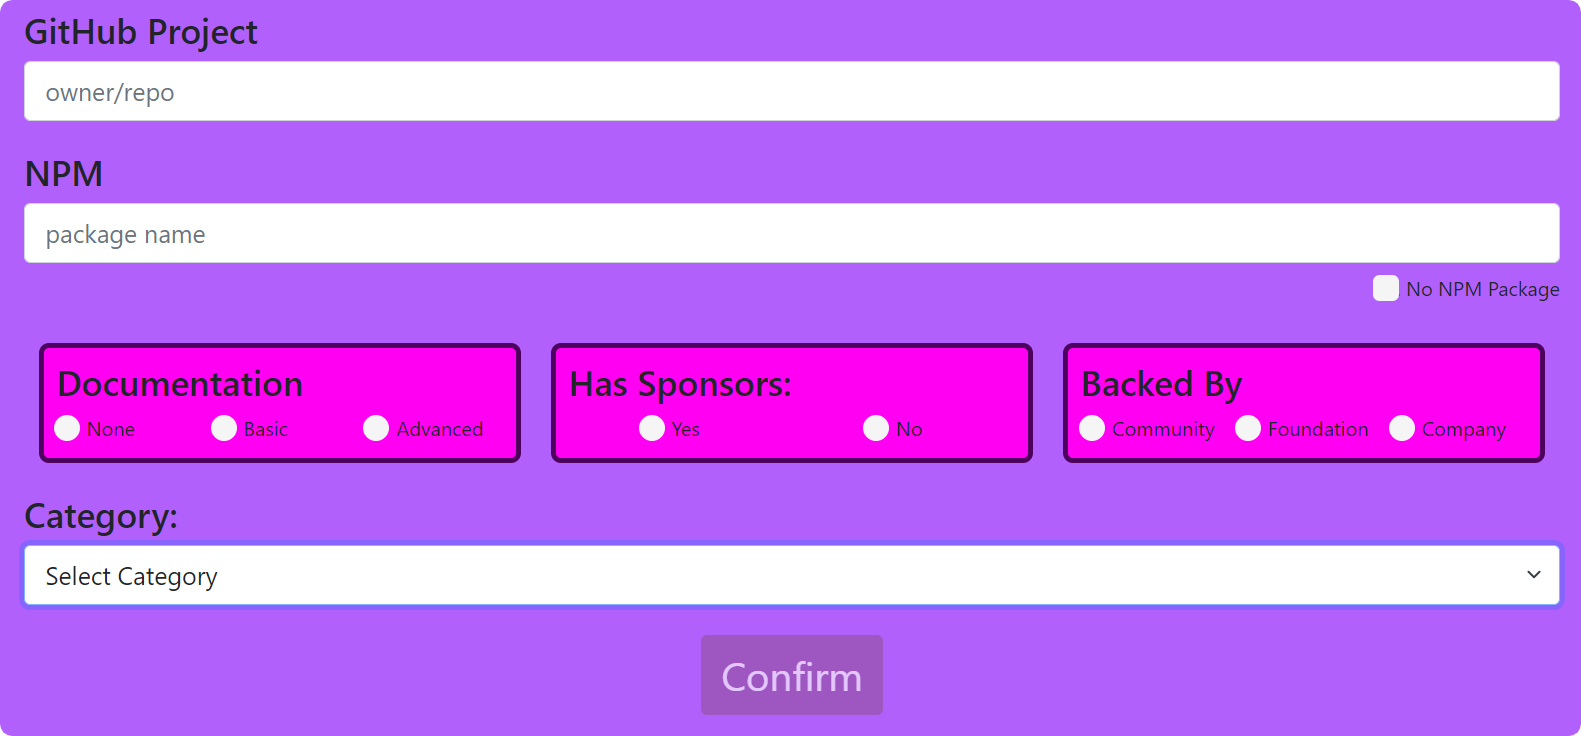
\includegraphics[scale=0.25]{figures/04/WebInterface.png}
    \caption{Web Interface}
    \label{abb:Web_Interface}
\end{figure}




% ----------------------------------------- Dokumentation ---------------------------------------- %
\subsection{Dokumentation}
Für die Dokumentation wurde \textit{README.md} bzw. eine externe Website überflogen und kategorisiert.
Bei der Qualität der Dokumentation wurde wie folgt bewertet:

\begin{itemize}[noitemsep]
    \item[0 =] keine Dokumentation
    \item[1 =] basis Dokumentation, rein textuell
    \item[2 =] Dokumentationen mit Demos oder Live Beispielen,
        Einführungsvideos oder ähnliches
\end{itemize}


% ------------------------------------------- Sponsoren ------------------------------------------ %
\subsection{Sponsoren}
Für jedes Projekt wurde geprüft, ob es Sponsoren hat. Auf der GitHub-Seite findet sich oft ein Link
zur Sponsoren Website oder alternativ gibt es meist in der \textit{README.md} bzw. auf der Website
des Projektes eine kurze Danksagung an die Sponsoren. Die Anzahl an Sponsoren bzw. die Einnahmen
durch Sponsoren wurden nicht beachtet, nur ob Sponsoren vorhanden sind.

\begin{itemize}[noitemsep]
    \item[0 =] hat keine Sponsoren
    \item[1 =] hat Sponsoren
\end{itemize}


\newpage %! newpage
% ------------------------------------------- Backed by ------------------------------------------ %
\subsection{Backed By}
Im nächsten Schritt wurde vermerkt wer hinter einem Projekt steht, hierbei wurde in drei Kategorien
eingeteilt:

\begin{itemize}[noitemsep]
    \item[0 =] Eines reinen Community Projektes unabhängig von Unternehmen. Beispiel: VueJS.
    \item[1 =] Von einer Stiftung wie OpenJS\footnote{\url{https://openjsf.org/}} unterstütztes oder
        entwickeltes Projekt.\\ Beispiel: NodeJS.
    \item[2 =] Projekte die von Unternehmen entwickelt werden, wie React von Facebook beispielsweise.
\end{itemize}

\noindent
Diese Information fanden sich entweder auf der GitHub-Page, Homepage des Projektes oder das Unternehmen
ist der Besitzer des Repositories.



% ------------------------------------------- Kategorie ------------------------------------------ %
\subsection{Kategorie}
Im letzten Schritt wurde das Projekt in eins der folgenden Kategorien zugeordnet: \\
Utility, UI, Application, Library, Framework, Test-Framework, Open-Core, API

\begin{multicols}{2}
    \begin{itemize}
        \setlength\itemsep{0em}
        \item Utility
        \item UI
        \item Application
        \item Library
        \item Framework
        \item Test-Framework
        \item Open-Core
        \item API
    \end{itemize}
\end{multicols}

% Erläuterung der Kategorien
\subsubsection*{Erläuterung der Kategorien}

\begin{itemize}
    \setlength\itemsep{0em}
    \item \textbf{Utility}, wurden Projekte kategorisiert, die nicht direkt in Projekte eingebaut
          werden, sondern als Tool verwendet werden. Beispiel: \texttt{shelljs/shelljs}\footnote{
              \url{https://github.com/shelljs/shelljs}}
    \item \textbf{Application}, sind eigenständige Produkte wie draw.io\footnote{
              https://github.com/jgraph/drawio}
\end{itemize}





% ------------------------------------------------------------------------------------------------ %
%                                                                                                  %
%                                   Automatisierte Datenerfassung                                  %
%                                                                                                  %
% ------------------------------------------------------------------------------------------------ %
\newpage %! newpage
\section{Automatisierte Datenerfassung}\label{sec:automatisierte_datenerfassung}

\todo{Im Text einbinden Architektur.}

Im zweiten Teil der Datenerfassung wurden weitere Daten automatisiert erhoben. Hierfür wurde die
GitHub API\footnote{\url{https://docs.github.com/en/rest}}, NPM
API\footnote{\url{https://github.com/npm/registry}} und für einige Daten Web-Scraping
verwendet.

Zu diesem Zweck wurde ein NodeJS Applikation geschrieben, die CSV aus dem ersten Schritt ausließt und
mithilfe der APIs und Web-Scraping eine neue CSV-Datei generiert. In den folgenden Unterkapiteln wird
aufgelistet welche Daten mittels welcher Methode gesammelt wurden.


% ----------------------------------- Daten aus der GitHub API ----------------------------------- %
\subsection{Daten aus der GitHub API}
Mittels der GitHub API wurden folgende Daten gesammelt:

\begin{itemize}[noitemsep]
    \item Anzahl der GitHub-Sternen
    \item Erstellungsdatum des Repositories
    \item Vorhandensein einer \textit{CODE\_OF\_CONDUCT.md}
    \item Vorhandensein einer \textit{CONTRIBUTING.md}
    \item Lizenz
    \item Anzahl der Commits in den letzten 12 Monaten
    \item Anzahl der Issues in den letzten 12 Monaten
\end{itemize}

% * GitHub_generalInfo
% * projectHealth
% * commitActivity
% * issues_PRs

% ------------------------------------- Daten aus der NPM API ------------------------------------ %
\subsection{Daten aus der NPM API}
Mit der NPM API wurden die Downloads der letzten 7 Tage abgefragt.

% * npm_downloads

% ---------------------------------- Daten aus dem Web-Scraping ---------------------------------- %
\subsection{Daten aus dem Web-Scraping}
Mithilfe von Web-Scraping wurden folgende Daten erfasst:

\begin{itemize}[noitemsep]
    \item Die Anzahl von \textit{UsedBy} auf der GitHub Page des Projektes.
    \item Anzahl der Gesamt-Commits auf dem default Branch
    \item Anzahl der Contributor
\end{itemize}

\subsubsection*{Anmerkung:}
Ein Contributor zählt nur dann als solcher, wenn dessen Commit entweder auf dem \textit{default}
oder \textit{gh-pages} Branch liegt. Commits auf anderen Branches werden nur dann gezählt, wenn ein
merge auf einen der vorherig erwähnten Branches stattfindet. Gleiches gilt für Commits \cite{GHapiDocsCommits}.

% * GitHub_usedBy
% * GitHub_Page
% * npm_dependants


% ----------------------------------- Nachbearbeitung der Daten ---------------------------------- %
\subsection{Nachbearbeitung der Daten}
\todoo{Nachdem erheben der Daten waren noch einige Schritte notwendig bevor die Daten analysiert werden
    konnten. Einige Projekte hatten die Lizenz \texttt{other}. Der Grund hierfür ist, dass die
    \texttt{LICENSE.md} nicht dem Standard Text entspricht. Ein Beispiel wäre die Lizenz von meteor\footnote{https://github.com/meteor/meteor/blob/devel/LICENSE}
    Alle als \texttt{other} gekennzeichneten Projekte wurden manuell geprüft und korrigiert.
    %
    Des Weiteren wurden Projekte ohne Lizenzen oder Lizenzen die nicht von der \textit{Open Source Initiative} zugelassene
    sind komplett aussortiert.
    %
    Nach dem gleichen Prinzip wurden Projekte kontrolliert die keine Contributing Guide bzw. kein Code of Conduct haben.
    Grund hierfür. GitHub erkennt das Vorhandensein dieser Dateien nur dann wenn diese im Hauptverzeichnis liegen.
    Andere Projekte wiederum haben ein Contributing Guide in der README.md oder auf deren Website. 
    % 9 Datensätze wurden korrigiert (Contributing) / 2 Datensätze wurden bezüglich (CoC) korrigiert
}




% ------------------------------------ Abbildung: Architektur ------------------------------------ %
\begin{figure}[]
    \centering
    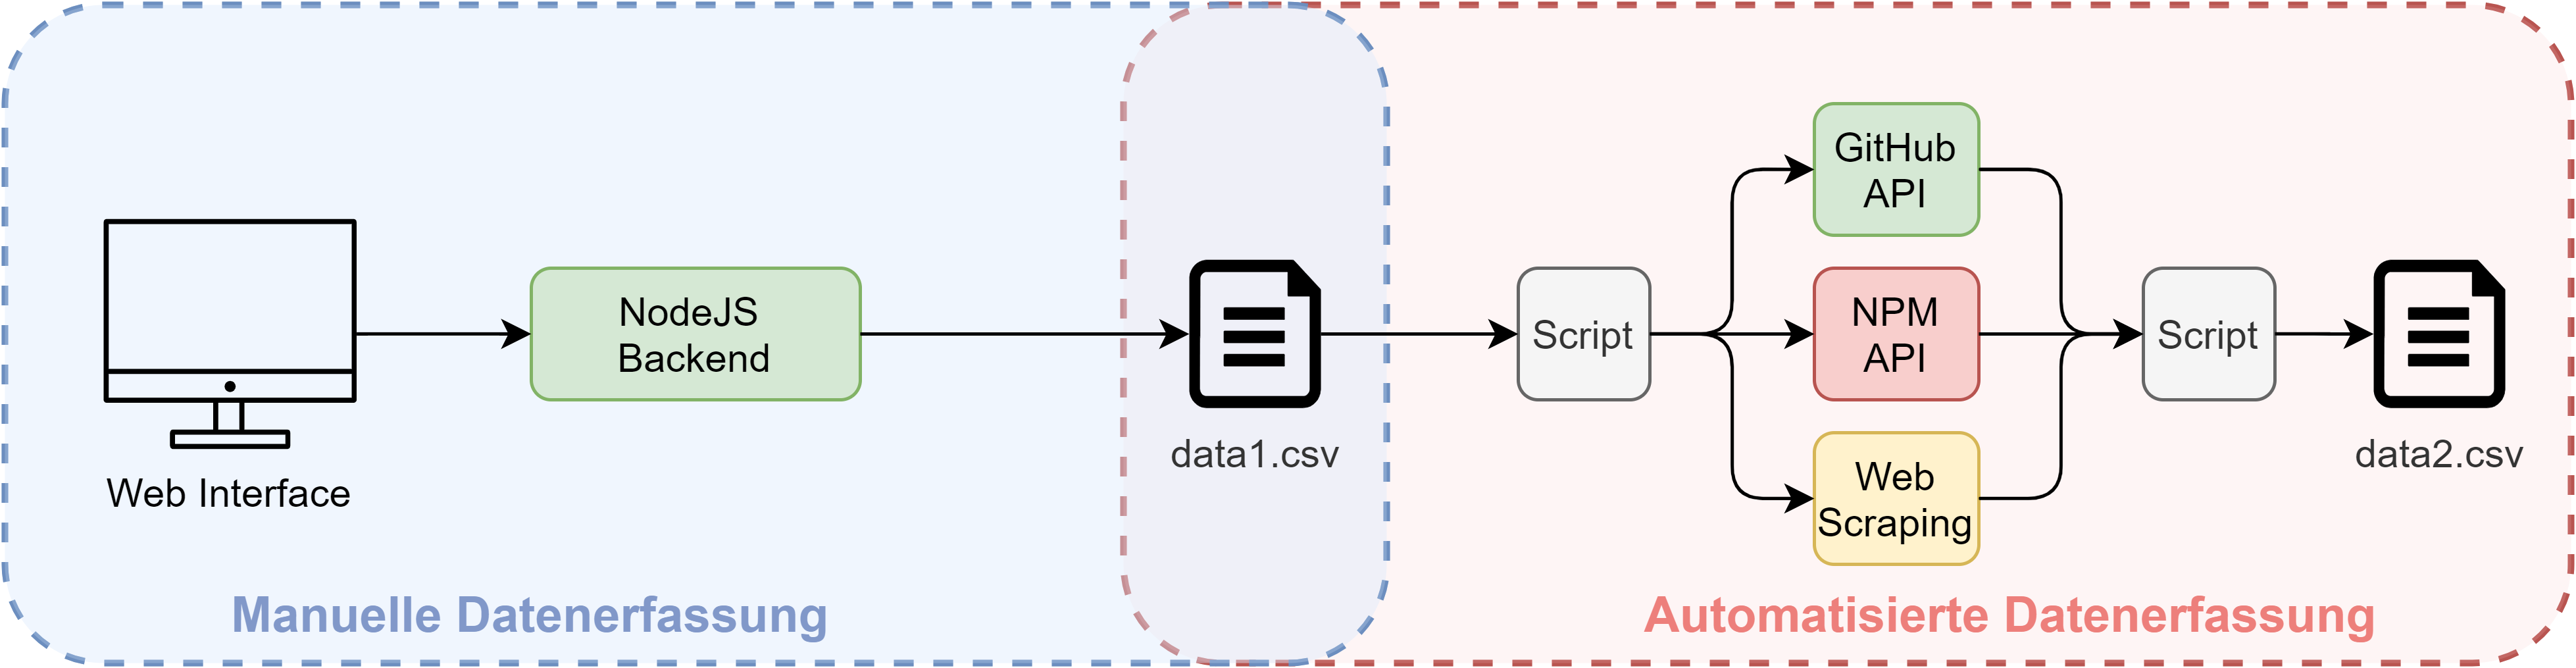
\includegraphics[scale=0.1]{figures/04/DatenerfassungArchitektur.png}
    \caption{Architektur}
    \label{abb:Architektur}
\end{figure}


% \section{Top 100 Projekte}\label{sec:top_100_projects}

% \todoo{Datenerhebubg der Top 100 Projekte, unabhängig von Programmiersprache. Ziel: Besseren eindruck
% über Lizenzen. Vorgehen: Wie zuvor auch, keine Tutorials etc. Abgespeckte Version weil die meisten
% "Funktionen" des Haversters abgeschaltet wurdens sind.}

% Hier wird die Regel "Nur JS" gebrochen, da das Ziel ist GH-Sterne in Relation zu den Lizenzen zu 
% vergleichen.